\chapter[Methods]{Methods}
This chapter outlines the modeling choices made when designing a pyroprocessing facility. 
The framework a model resides in is a key design choice, and we cover why \Cyclus provides
a productive environment for designing and testing this facility. In the \Cyclus framework we
design the Pyre archetype as a generic modular facility using material balance areas and identifying key signatures and observables. Leveraging this information, we design a diverter class to integrate within Pyre. This diverter tracks and alters operational parameters to mimic
the actions of shadow fuel cycles.

\section{Cyclus}

\Cyclus is a modular, agent-based nuclear fuel cycle simulator that models the flow of material through user-defined nuclear fuel cycle scenarios. \Cycamore, the CYClus 
Additional MOdules REpository, provides common facility archetypes (separations, enrichment, reactor, etc.) \cite{carlsen_cycamore_2014}. 
The \Cyclus framework provides benefits compared to other fuel cycle simulators, some being the open source nature, modular capabilities, and use of agents.
Customizable agents populate simulations, allowing for a diverse use case. Exact isotopes are dynamically tracked between facilities in discrete time steps \cite{huff_fundamental_2016}.
Isotope tracking is a key aspect of \Cyclus that we will use for signatures and observables, in addition to allowing burn-up calculations in more complex fuel cycle scenarios.

\subsection{Open Source}

Many fuel cycle simulators have restrictive licenses such as ORION, VISION, or COSI. This restricts
nuclear fuel cycle simulator use and development in academia, therefore a tool such as \Cyclus fills a necessary gap. The \Cyclus framework relies on
free libraries and open development that allows continuous contributions from various universities and fields of research. This increased accessibility allows
more diverse use and expansion of the simulator as seen with codes like CyBORG and Bright-Lite \cite{skutnik_cyborg:_2016,schneider_integrated_2016}.

\subsection{Reproducibility}
Cooperation and collaborative development are a major part of open source development. This is maintained through code reviews. These reviews are conducted by peers,
and are used to check code style, documentation, and functionality. As such, any addition to open source code in particular should be well tested.
Thorough testing allows concurrent or future developers to maintain and expand the project while ensuring all capabilities are maintained. Following these guidelines, we
implement a number of tests verifying trade capability and sub-process physics to ensure reproducibility. The details of these verifications will be explained further in Chapter 3.

\subsection{Modular}

The modularity of \Cyclus also contributes to the customizability of fuel cycle scenarios. Rather than having locked material connections between facilities, the modular
\Cyclus framework allows easy implementation of new connections. This is handled through the use of a dynamic resource exchange (DRE) in the \Cyclus kernel \cite{gidden_agent-based_2015}. 
The DRE uses a system of material offers and requests to find the best connections at each time step. Figure \ref{fig:cyc-api} demonstrates how the agent API is used to mediate
the \Cyclus kernel DRE and the implementation of each agent.  

\begin{figure}
	\centering
	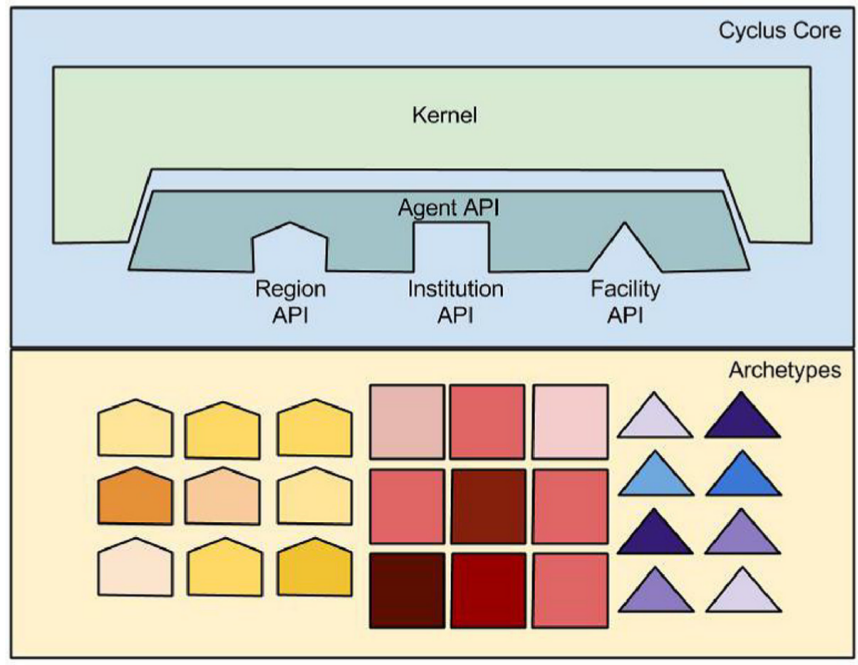
\includegraphics[width=0.7\linewidth]{images/cyclus-core}
	\caption{Visualization of the \Cyclus API for modular facilities, regions, and institutions \cite{huff_fundamental_2016}.}
	\label{fig:cyc-api}
\end{figure}

The structure seen in Figure \ref{fig:cyc-api} is largely responsible for the potential breadth of agent types of varying fidelity. Provided new agents have the appropriate material trade offers and requests,
facilities can be designed to any required fidelity.

\subsection{Archetypes}

Agents contain a hierarchy of \emph{regions, institutions, and facilities} such that \emph{regions} hold one or more \emph{institutions}. Similarly, \emph{institutions}
control \emph{facilities} necessary for the actual fuel cycle. For this work, we are most interested in the implementation of \emph{facilities} - particularly how they are defined.
Nuclear fuel cycles contain multiple variations of the same facility requiring a diverse collection of pre-designed facility process models, known as \emph{archetypes}.
These archetypes are used to define the physics and behavior of specific facility types such as reactors, reprocessing, enrichment, etc. Archetypes with pre-defined parameters are referred
to as prototypes (an AP1000 for example is a prototype). Furthermore, facilities are prototypes that have been given specific data such as deployment time, location, lifetime, etc.

\section{Pyre}

This thesis work included original design and implementation of \Cyclus facility archetype, Pyre, which has various capabilities. Pyre was designed such that multiple potential pyroprocessing facilities can be modeled at medium fidelity. To accomplish this, and improve upon
the lower fidelity of the separations archetype found in \Cycamore, Pyre separation efficiencies is informed by higher fidelity models including SSPM and AMPYRE \cite{cipiti_modeling_2012,maggos_update_2015}. The below Figure \ref{fig:flowchart} incorporates material balances for each sub-process and highlights some key parameters Pyre
requires the user to provide in the input file or monitor for diversion.

\subsection{Structure of Pyre}

The Pyre archetype separates each sub-process (voloxidation, electroreduction, electrorefining, and electrowinning) to be handled independently, letting the user determine which aspects are necessary for their facility. Pyre takes this approach to improve handling of various waste streams. Ceramic waste must go through the electroreductor, whereas metallic fuel can go straight into the electrorefiner \cite{michael_f._simpson_developments_2012}. This reduces reprocessing time, as Pyre does not force redundant processes.

\paragraph{Governing Pyre Class} \mbox{}\\
The archetype treats each sub-process as optional and independent, letting the user determine which aspects are necessary for their facility. Each sub-process handles its own diversion and material tracking. The streams produced from these processes are sent further through the facility, and the streams are recorded. Waste streams are
used to verify nominal operation before being traded to a storage facility. Product streams are further refined by each sub-process until the fuel fabrication stage.
The pure uranium stream and U/TRU stream are then offered up for trade with a fuel fabricator.

\FloatBarrier

\begin{figure}[h]
	\centering
	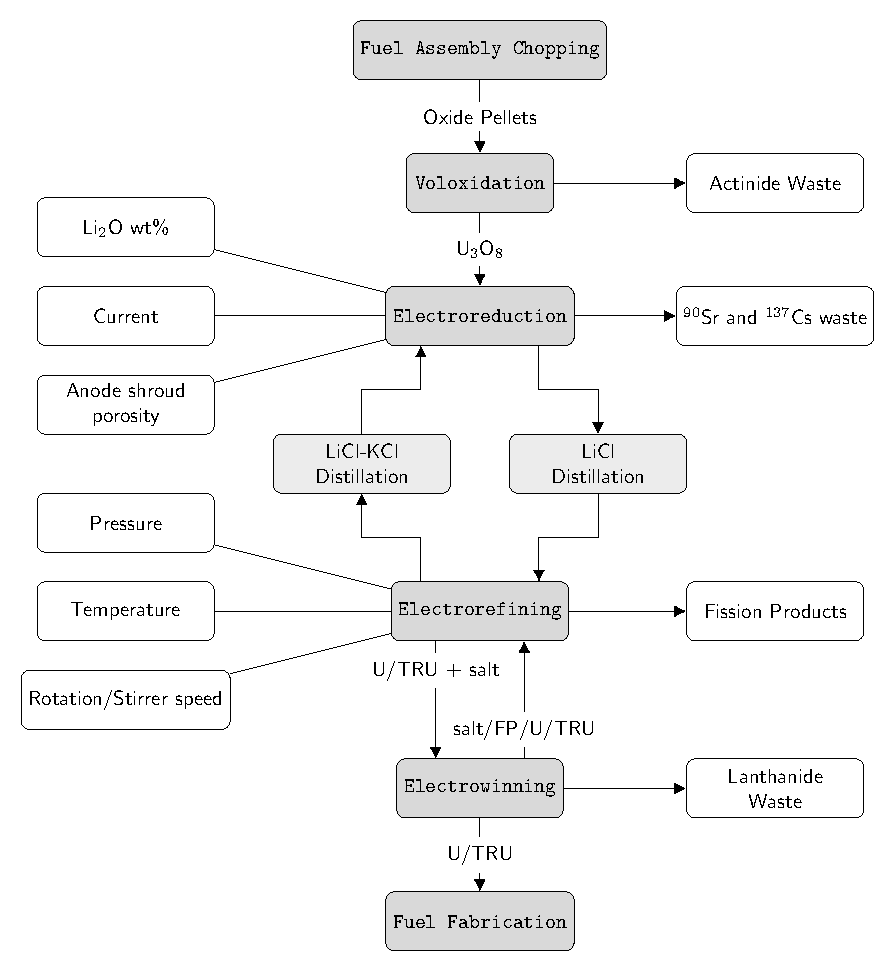
\includegraphics[width=0.9\linewidth]{images/flowchart}
	\caption{Pyre material flowchart \cite{borrelli_approaches_2017}.}
	\label{fig:flowchart}
\end{figure}

\FloatBarrier

\section{Signatures and Observables}

Before constructing a pyroprocessing archetype, appropriate signatures and observables must be determined to set as our input parameters. To identify signatures and observables 
found in a variety of pyroprocessing plants, we expand upon what was discussed in chapter 1 by looking at experimental data from electrochemical plants. The primary resources are from 
INL, KAERI, and ANL \cite{lee_korean_2011,flowsheet_1998,michael_f._simpson_developments_2012,li_electrorefining_2005}. We break up these signatures and observables into two distinct categories: direct and indirect, corresponding to signatures and observables, respectively. If the inspector has direct access to material these are referred to as signatures, whereas, indirect monitoring, such as
power draw or thermal imaging, represent a lower level of access. 

Potentially trackable signatures and observables include truck deliveries and  power draw  \cite{Hou_2016,Yilmaz_2016}. This list is expanded upon in Table \ref{tab:params} to include pyroprocessing parameters. For this work we narrow down the list to more facility specific parameters rather than observables like the parking lot or truck movement. We also use this table
to determine the most common operational settings such as temperature, pressure, current and flow rate.

\begin{table}[h]
	\centering
	\begin{tabularx}{0.9\linewidth}{llcr}
		\hline
		\textbf{Sub-process} & \textbf{Parameters} & \textbf{S \& O} & \textbf{Refs} \\
		\hline
		Voloxidation & Volume & Tritium & \cite{jubin_spent_2009} \\
		& Oxidant & $^{14}$C & \cite{flowsheet_1998} \\
		& Flow Rate &  $^{129}$I &  \\
		& Temperature & $^{85}$Kr &  \\
		& Time & Actinides & \\ \hline
		Electroreduction & Volume & $^{90}$Sr & \cite{borrelli_approaches_2017} \\
		& Batch Size & $^{135}$Cs & \cite{flowsheet_1998} \\
		& Li$_2$O wt\% & $^{137}$Cs & \cite{choi_electrochemical_2015} \\
		& Current & Power Draw & \cite{lee_korean_2011} \\
		& Porosity & Shipments & \cite{lee_modeling_2016} \\
		& Distillation Speed & Throughput & \\ 
		& Time & & \\ \hline
		Electrorefining & Volume & Fission Products & \cite{lee_advanced_2008} \\
		& Time & Power Draw & \cite{lee_korean_2011} \\
		& Material & Waste Salt & \cite{flowsheet_1998} \\
		& Anode Rotation & Vacuum Pressure & \cite{koyama_development_2012} \\
		& Stirrer Speed & Temperature & \cite{kim_development_2013} \\
		& Pressure & Throughput & \\
		& Temperature & & \\ \hline
		Electrowinning & Current & Power Draw & \cite{flowsheet_1998} \\
		& Shroud Material & Cadmium Waste & \cite{lee_korean_2011} \\
		& Time & Fission Products & \cite{borrelli_approaches_2017} \\
		& Flow Rate & Lanthanides & \\
		&  & $^{135}$Cs & \\
		&  & $^{137}$Cs & \\ \hline
		Facility & Throughput & Shipments & \\
		& Batch Size & Parking Lot & \\
		& & Thermal Image & \\
		\hline
	\end{tabularx}
	\caption {Archetype inputs and signatures \& observables at each sub-process.}
	\label {tab:params}
\end{table}

\subsection{Material Balance}
We take a material balance area over each sub-processes using the signatures and observables identified in Table \ref{tab:params}. 
These balance areas are shown through flowcharts describing operational parameters in green, and signatures and observables in red. 

\paragraph{Voloxidation} \mbox{}\\
\gls{LWR} fuel must be treated and separated before proceeding with electrochemical processes. Uranium dioxide heated to 
500$^{\circ}$C is converted to $U_3O_8$ while noble gases, carbon, and tritium are collected to decay in storage. 
Actinides are also converted to their stable oxide forms and a majority are removed \cite{flowsheet_1998,jubin_spent_2009}. 
Heating uranium dioxide above 800$^{\circ}$C increases voloxidation throughput.
Cycling oxidants between H$_2$ and air also improves the U$_3$O$_8$ reaction rate \cite{jubin_spent_2009}.

\begin{figure}[h]
	\centering
	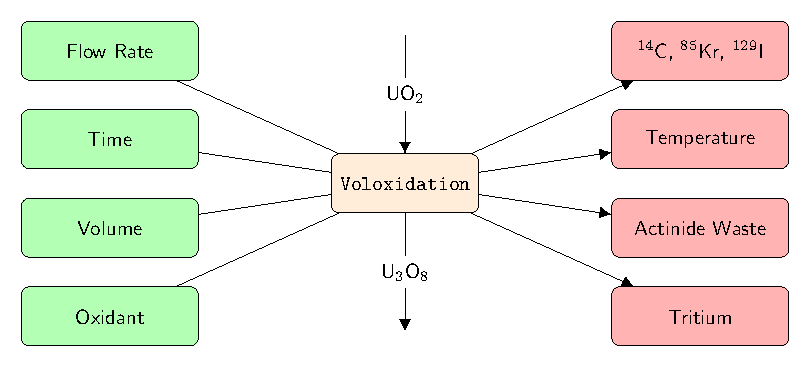
\includegraphics[width=0.9\linewidth]{images/volox}
	\caption{Voloxidation material balance area \cite{jubin_spent_2009}.}
	\label{fig:volox}
\end{figure}

\paragraph{Electroreduction} \mbox{}\\ 
Yellowcake, created in voloxidation, enters the cathode, a negatively charged metal basket. 
A current density between 100 and 500 mA/cm$^2$ is applied to the anode in a molten LiCl salt. 
The electrolytic reduction process primarily results in diffusion of Cs, Ba and Sr, along with reduction and conversion of Zr into metallic form \cite{choi_electrochemical_2015,flowsheet_1998}.
Electroreduction can further improve its throughput by adding Li$_2$O as a catalyst; this catalyst also prevents dissolution 
of the anode \cite{choi_electrochemical_2015}. Since Li$_2$O is used to speed up the reaction,
the operators could add more oxide than reported to \gls{IAEA}. More frequent shipments 
of lithium oxide can be tracked as an observable to match records.

\begin{figure}[h]
	\centering
	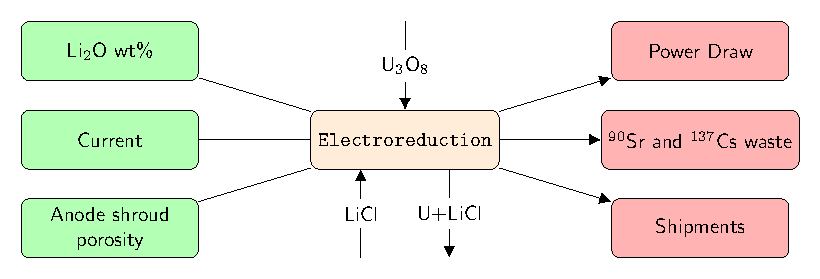
\includegraphics[width=0.9\linewidth]{images/reduction}
	\caption{Reduction material balance area \cite{lee_advanced_2008}.}
	\label{fig:reduction}
\end{figure}

\paragraph{Electrorefiner} \mbox{}\\
Once in metallic form, electrorefining electrochemically separates uranium and TRUs for fuel fabrication.
The uranium and salt mixture from reduction is fed into an anode basket suspended in a graphite cathode. 
A LiCl-KCl eutectic is used as an electrolyte above 500$^{\circ}$C \cite{flowsheet_1998,lee_korean_2011}. 
Uranium dissolves at the anode to recombine at the cathode as metallic uranium.
Waste TRUs and lanthanides are in a soluble chloride form  while fission products and cladding remain in the anode
basket. Finally, actinides and fission products are removed from the cladding electrochemically \cite{lee_korean_2011}.

Lee et al. \cite{lee_advanced_2008} show decreasing system pressure improves removal efficiency. 
Temperature, however, exhibits the opposite effect: as temperature decreases so does salt removal. This comes into effect 
particularly depending on instrumentation and containment material choice \cite{lee_advanced_2008}. 
Iron, for example, limits operating temperature because a eutectic forms at 725$^{\circ}$C \cite{chapman_revision_1984}.
In facilities where iron equipment is present, temperatures are limited to 700$^{\circ}$C, hindering efficiency. 
Cathode arrangement and anode rotation speed also affect the collection of uranium 
dendrites \cite{lee_advanced_2008}.

\begin{figure}[h]
	\centering
	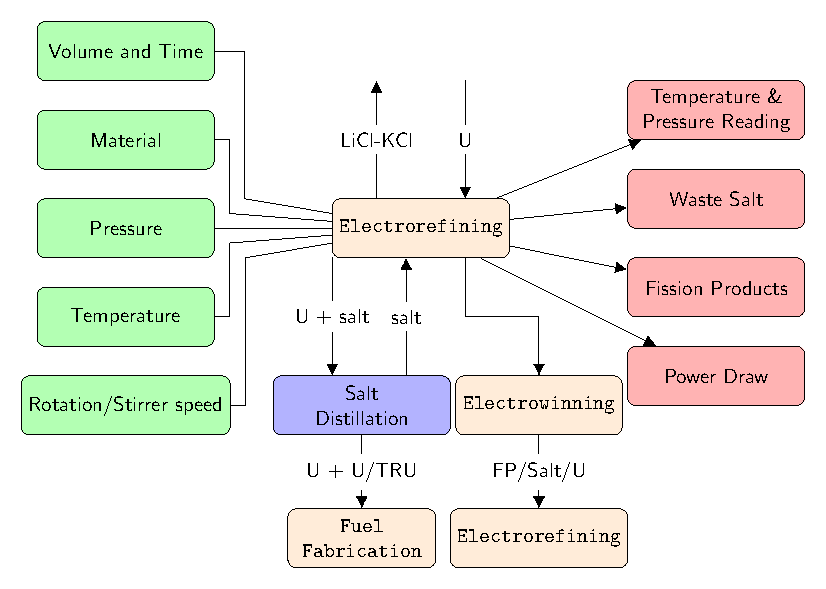
\includegraphics[width=0.85\linewidth]{images/refining}
	\caption{Refining material balance area \cite{lee_advanced_2008}.}
	\label{fig:refining}
\end{figure}

The electrorefining process also produces a fission product waste stream which requires monitoring. 
The following products are produced and tracked in Pyre at this step: Tc, Ag, Pd, Rh, Ru, Mo, and Zr \cite{flowsheet_1998}. 
Uranium and \gls{TRU} product streams separated at this stage are sent to fuel fabrication, while the remaining salt is reformed as an oxidant and recirculated.
Separation efficiencies are taken after recirculation and treated as a once-through cycle. 

\paragraph{Electrowinner} \mbox{}\\
Molten salt containing \glspl{TRU} from electrorefining is separated through electrowinning. This process separates trace uranium quantities, lanthanides and fission products. 
At 500$^{\circ}$C there is approximately 99 wt\% reduction in actinides and lanthanides \cite{flowsheet_1998}. 
Throughput also depends on material choice for the inert electrodes, impacting separation 
efficiency \cite{koyama_development_2012}. A shroud surrounds the anode to provide a path for O$^{2-}$ ions to the anode and 
prevent Cl$_2$ from corroding the anode \cite{kim_development_2013,choi_electrochemical_2015}. Optimum operating current 
depends on material choice for the anode shroud since a nonporous shroud limits ion pathways to the anode contact points.
Higher porosity corresponds to free ion paths and a higher current. Increased currents reduce the separation time for electroreduction and electrowinning \cite{choi_electrochemical_2015}.

\begin{figure}[h] 
	\centering
	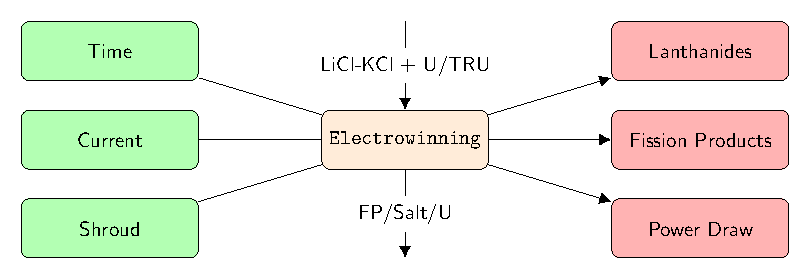
\includegraphics[width=0.8\linewidth]{images/winning}
	\caption{Winning material balance area.}
	\label{fig:winning}
\end{figure}

\subsection{Waste Forms}

Waste from pyroprocessing plants exists in three main waste streams in which IAEA can directly measure their \emph{signatures}. Monitoring signatures require direct access to the waste streams.
These techniques vary depending on the waste form. Leading approaches include non-destructive assay, multiplicity counting, and a plutonium to curium ratio measurement \cite{lee_determination_2012,noauthor_non-destructive_nodate}.

\paragraph{Diverter} \mbox{}\\
Figure \ref{fig:diverttype} shows the difference between nefarious diversion, in gray, and operator diversion, in orange. The gray line shows normal operation where diversion occurs
through the shipment, and can be detected by a discrepancy in shipment records. The more difficult case to handle, shown in orange, imagines an inside man altering operational settings
to increase product over reported quantities. The scenario we are concerned with is operator diversion; we wish to determine the most important points in the plant to monitor for potential
diversion. A side effect of this goal is that we must be able to detect diversion by changing key operational settings.

\FloatBarrier

\begin{figure}[h]
	\centering
	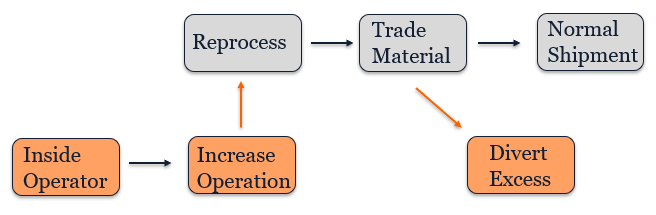
\includegraphics[width=0.8\linewidth]{images/westphal-diversion}
	\caption{A flowchart demonstrating the main forms of material diversion.}
	\label{fig:diverttype}
\end{figure}

\Cyclus does not natively handle diversion from inside facilities as required for the goals for Pyre. We implemented a higher fidelity diversion model through the
diverter class to handle operator and nefarious diversion. This class is specific to the Pyre archetype currently, as the diversion facility must be set up to allow it.
The diverter class' goal is to inform the Pyre facility what parameters are being changed to divert material. The algorithm used for this can be seen in Figure \ref{fig:divflow}
which inputs the sub-process that contains an inside man, the parameters he has access to, and how much material he wishes to divert. The diverter directs this information to the
appropriate sub-process which then uses a bisection function to determine the parameter value associated with the new product.

\FloatBarrier

\begin{figure}[h]
	\centering
	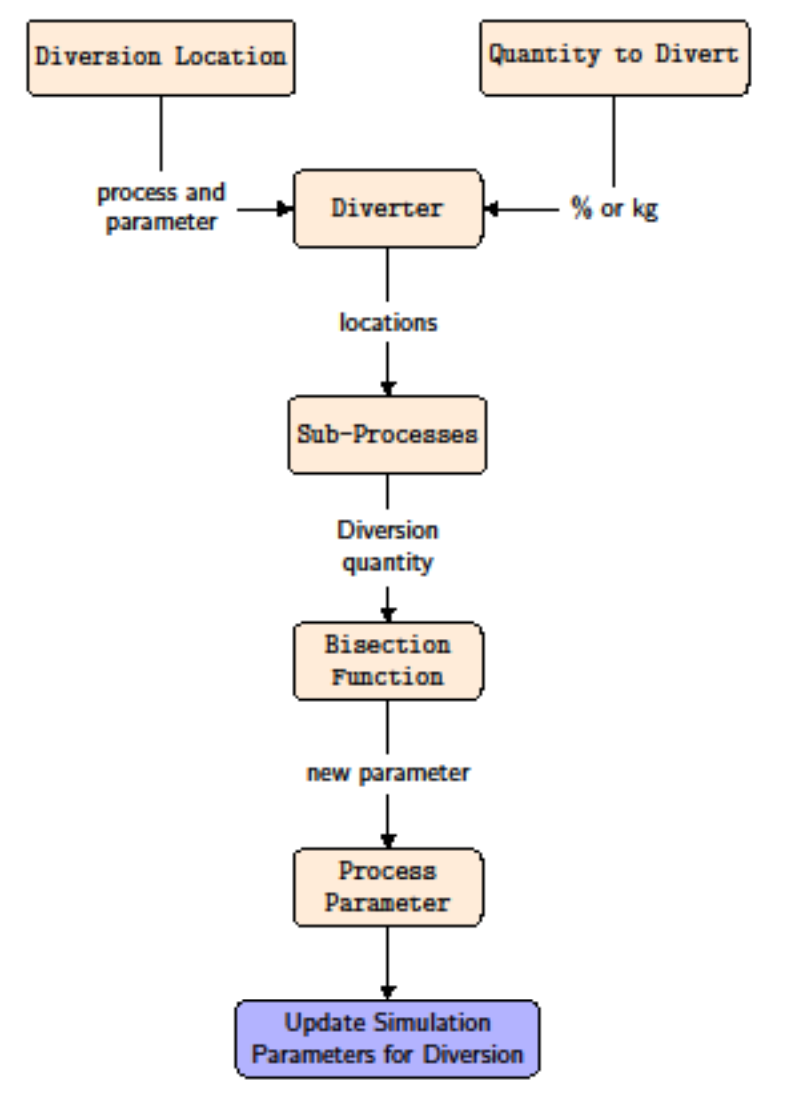
\includegraphics[width=0.65\linewidth]{images/divertflow}
	\caption{Pyre diverter class flowchart.}
	\label{fig:divflow}
\end{figure}

\subsection{User Input}
Pyre, as with all \Cyclus archetypes, is fully configurable through the text-based input file. The input consists of the operational settings shown in Table \ref{tab:params}
and the separation efficiency for each isotope. The efficiency input for each sub-process corresponds to that facility's ideal state. Operational settings act as a capacity factor,
reducing the overall efficiency to match those seen in test facilities. This input structure allows users to follow predefined example facilities, or input their own separation
efficiencies. As a result of this work, input files for PRIDE, INL, and ANL based facilities have been generated. However, a user can also input their own parameter relationship equations
if those provided do not accurately reflect their facility model.